\section{System Design}
\begin{frame}{Overview}
   \tableofcontents[sectionstyle=show/hide, hideothersubsections]
\begin{center}
  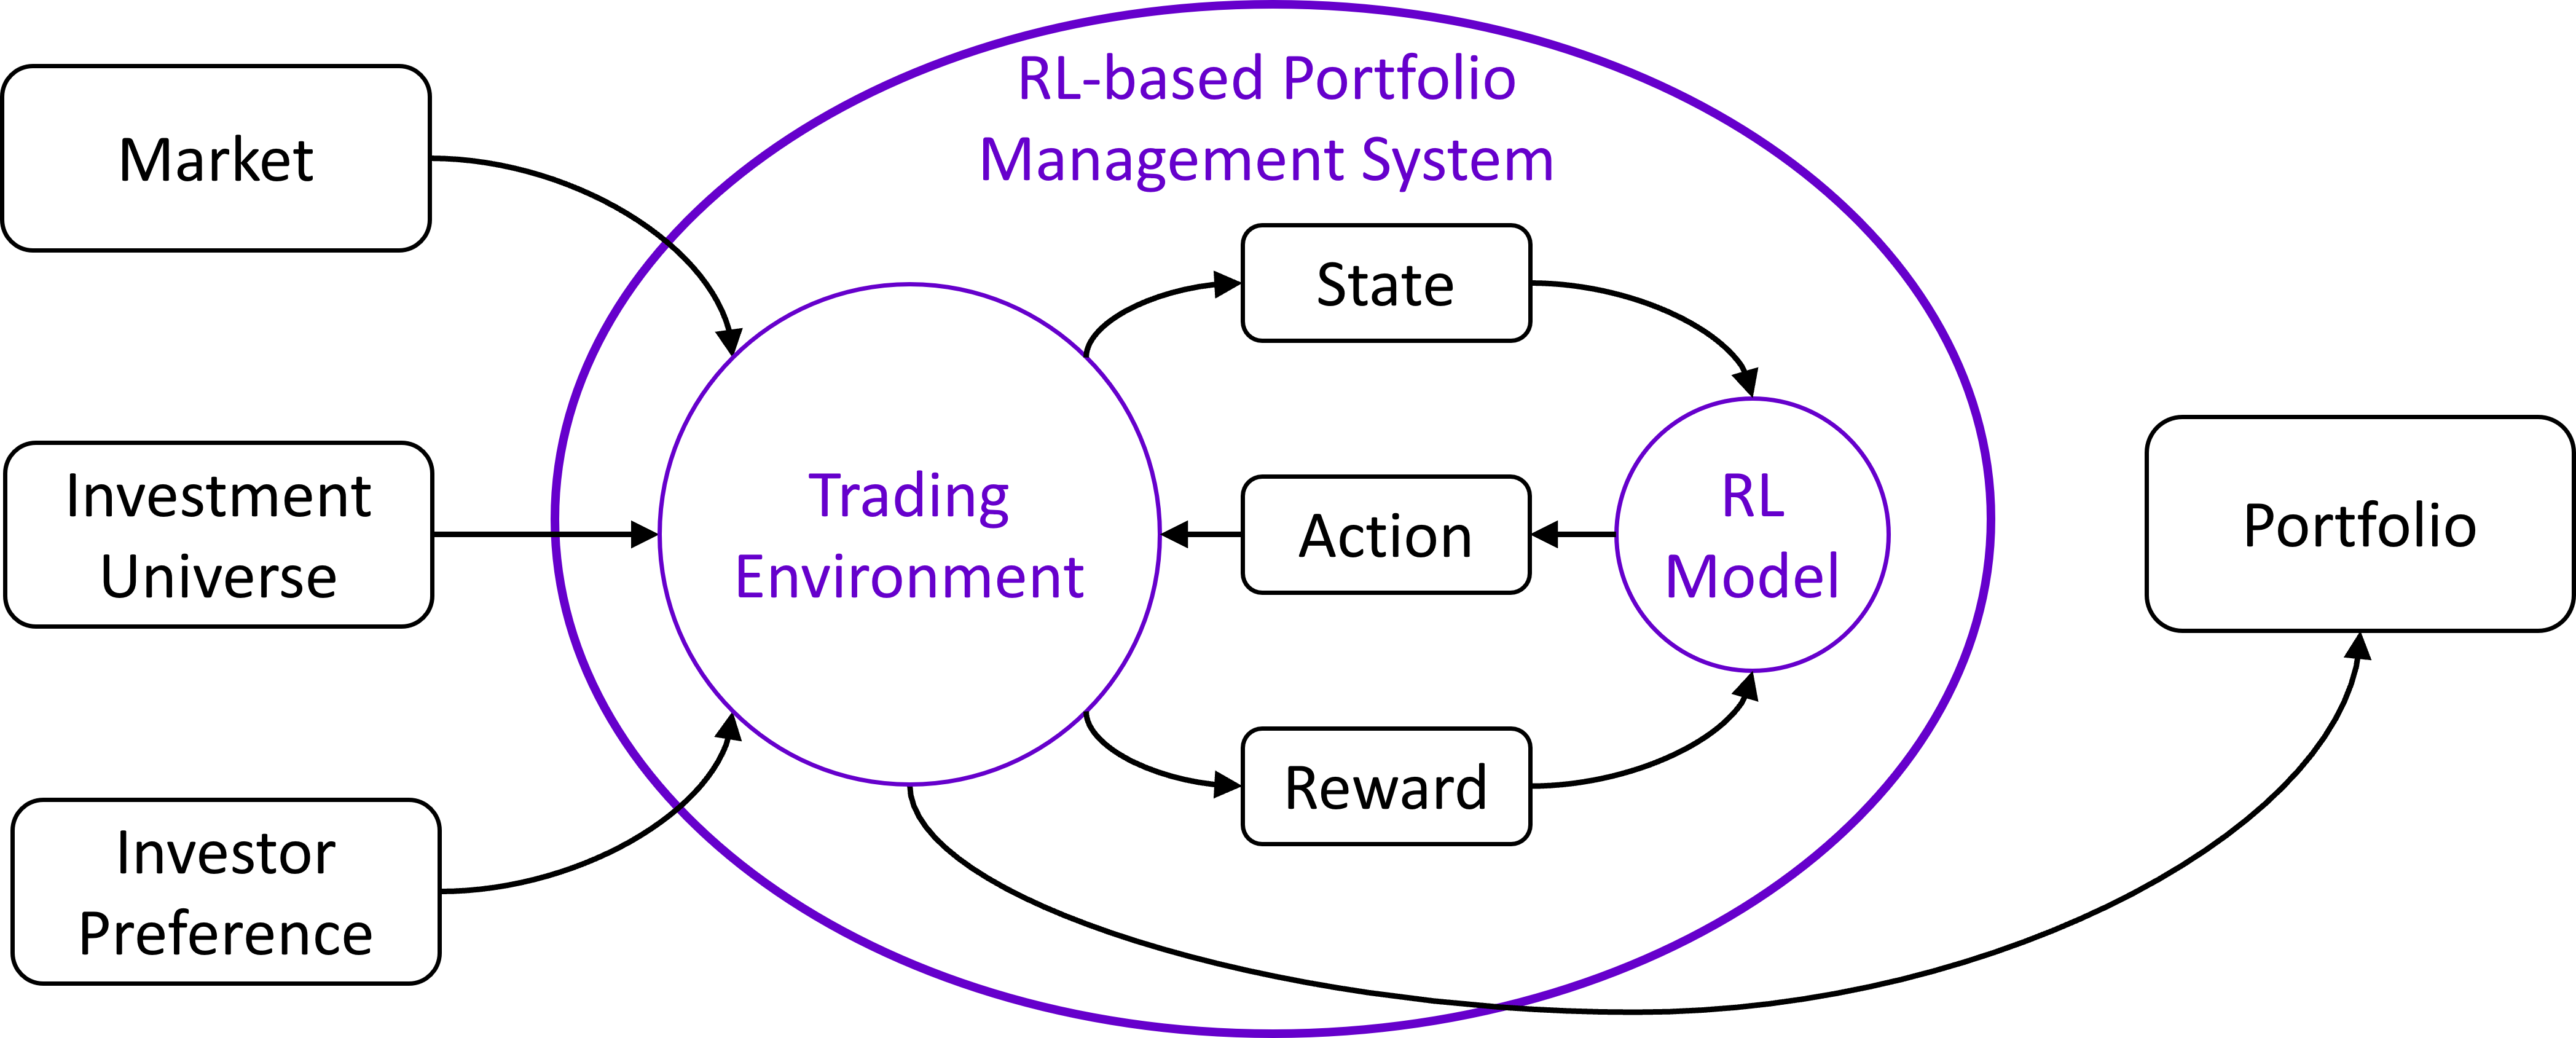
\includegraphics[width=10cm]{images/context_diagram.png} 
\end{center}
\end{frame}


\subsection{Market Features}
\begin{frame}{Market Features}
    \begin{block}{Objective}
        Select features to represent the status of the market.
    \end{block}
\centering
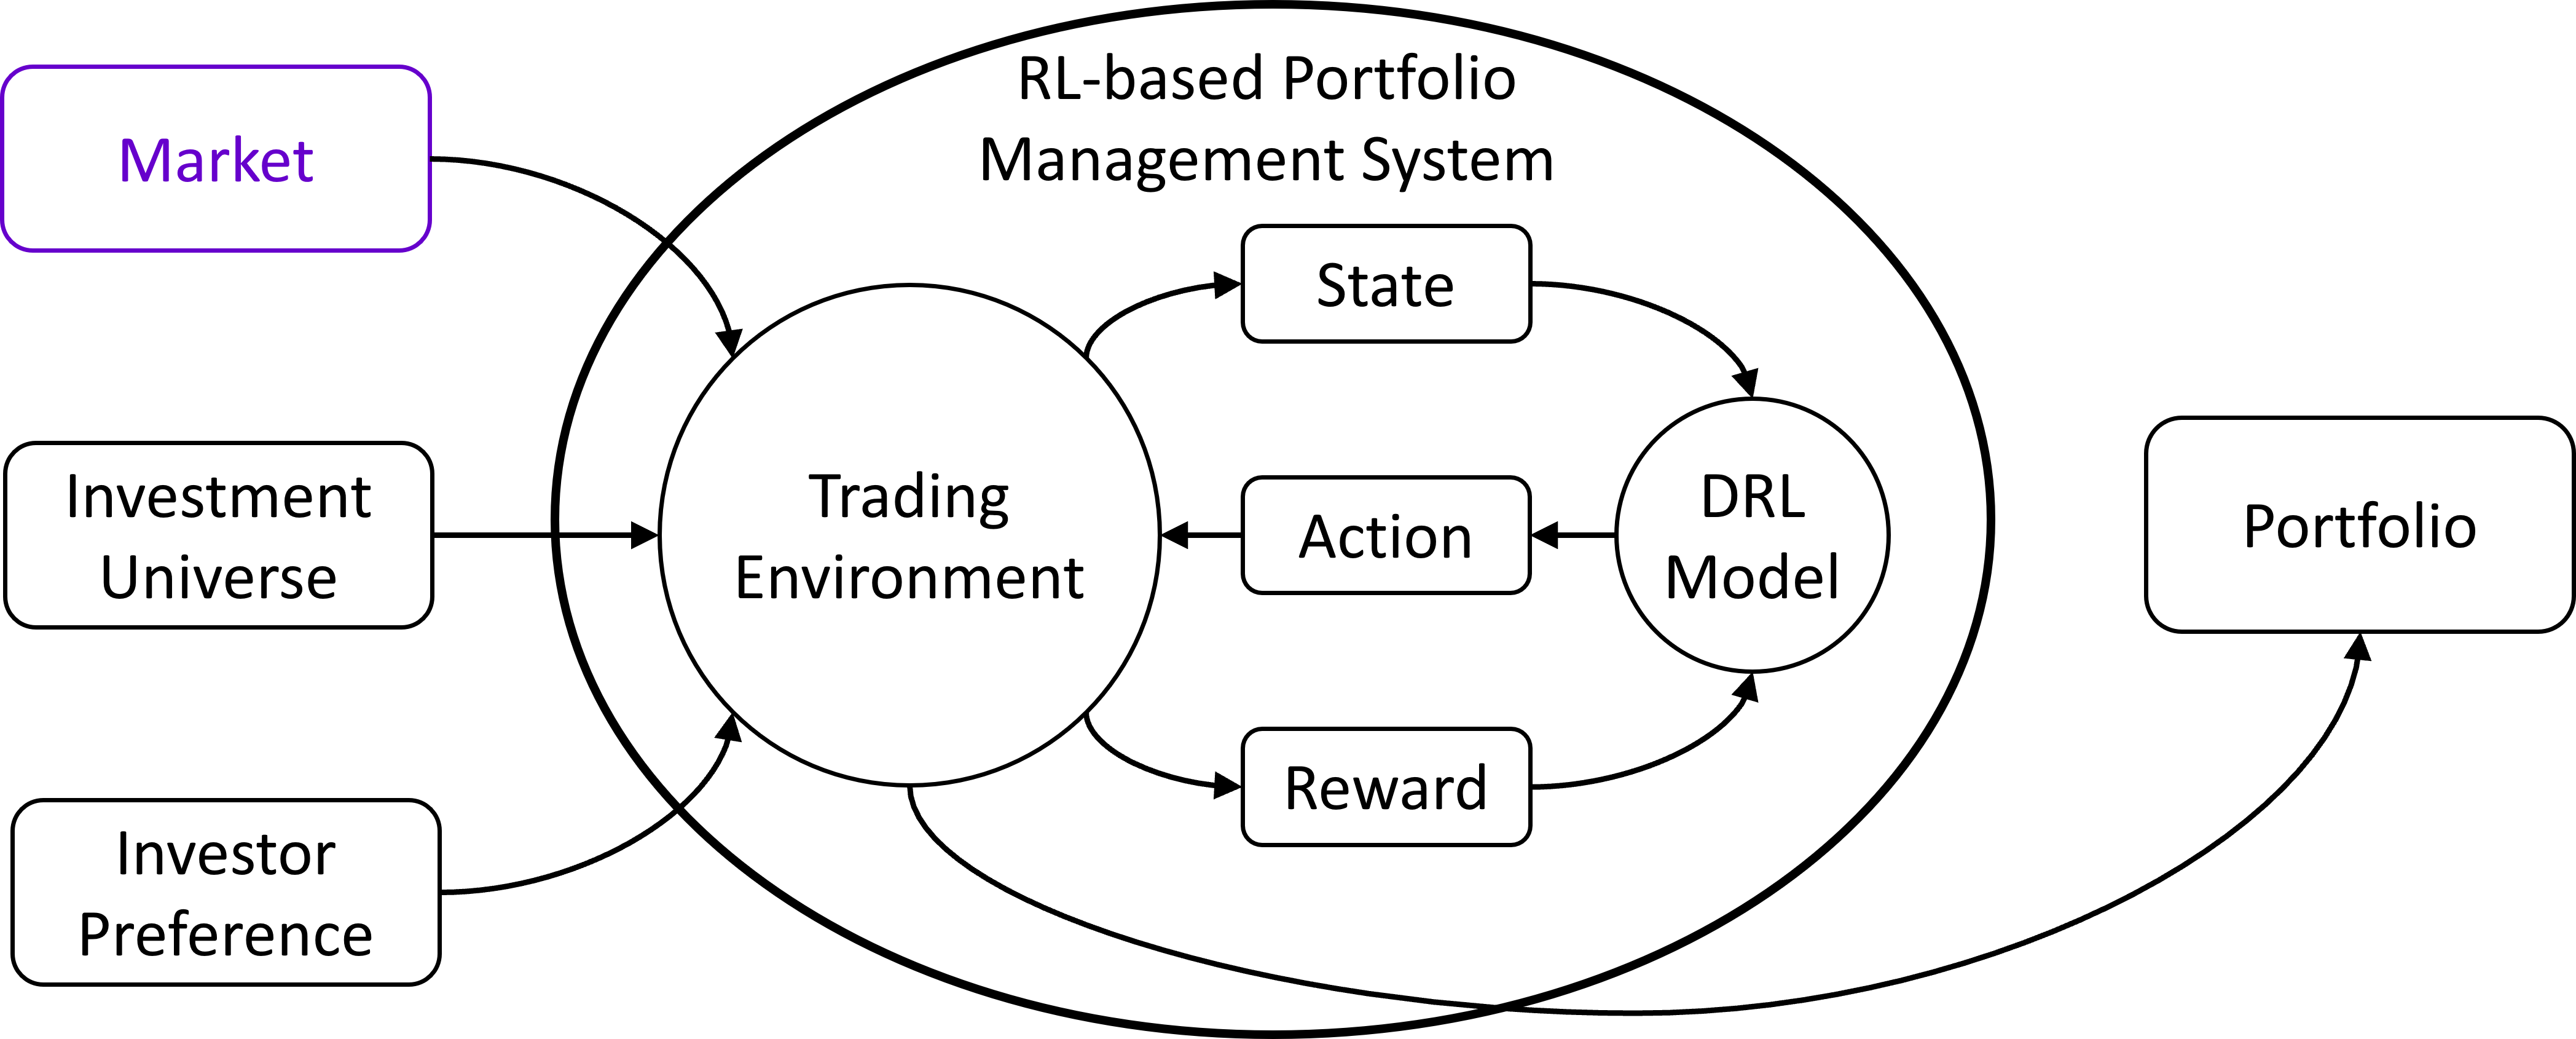
\includegraphics[width=10cm]{images/market.png}

\end{frame}

\begin{frame}{Market Features}
\begin{block}{Structured information}
\begin{itemize}
    \item Interest rates
    \item Commodity prices
    \item Currency exchange indexes
    \item Other Indexes
\end{itemize}
\end{block}
\begin{block}{Stationary data}
   Use directly as features
\end{block}
\begin{block}{Non-stationary data}
    Use statistics measures among 5, 20, and 60 days as features, including standard deviation, skewness, and kurtosis.
\end{block}
\end{frame}

\begin{frame}{Market Features}
\footnotesize
\begin{tabular}{|| c| c | c||}
\hline
Description & Categories & Stationary \\ \hline \hline
5-Year Treasury Constant Maturity Rate & Interest Rates  & Yes \\ \hline
10-Year Treasury Constant Maturity Rate & Interest Rates & Yes \\ \hline
30-Year Treasury Constant Maturity Rate & Interest Rates & Yes \\ \hline
5-Year Breakeven Inflation Rate & Interest Rates & Yes \\ \hline
10-Year Breakeven Inflation Rate & Interest Rates & Yes \\ \hline
Crude Oil Prices: Brent - Europe &  Commodities & No \\ \hline
Gold Prices &  Commodities & No \\ \hline
CBOE Volatility Index (VIX) &  Indexes & No \\ \hline
US Dollar Index (USDX) &  Currencies & No \\ \hline
\end{tabular}
\end{frame}



\newcommand\mynum[1]{{\renewcommand{\insertenumlabel}{#1}%
      \usebeamertemplate{enumerate item}}}



\subsection{Investment Universe}
\begin{frame}{Investment Universe}
    \begin{block}{Objective}
        Pick available investments for the portfolio.
    \end{block}


\centering
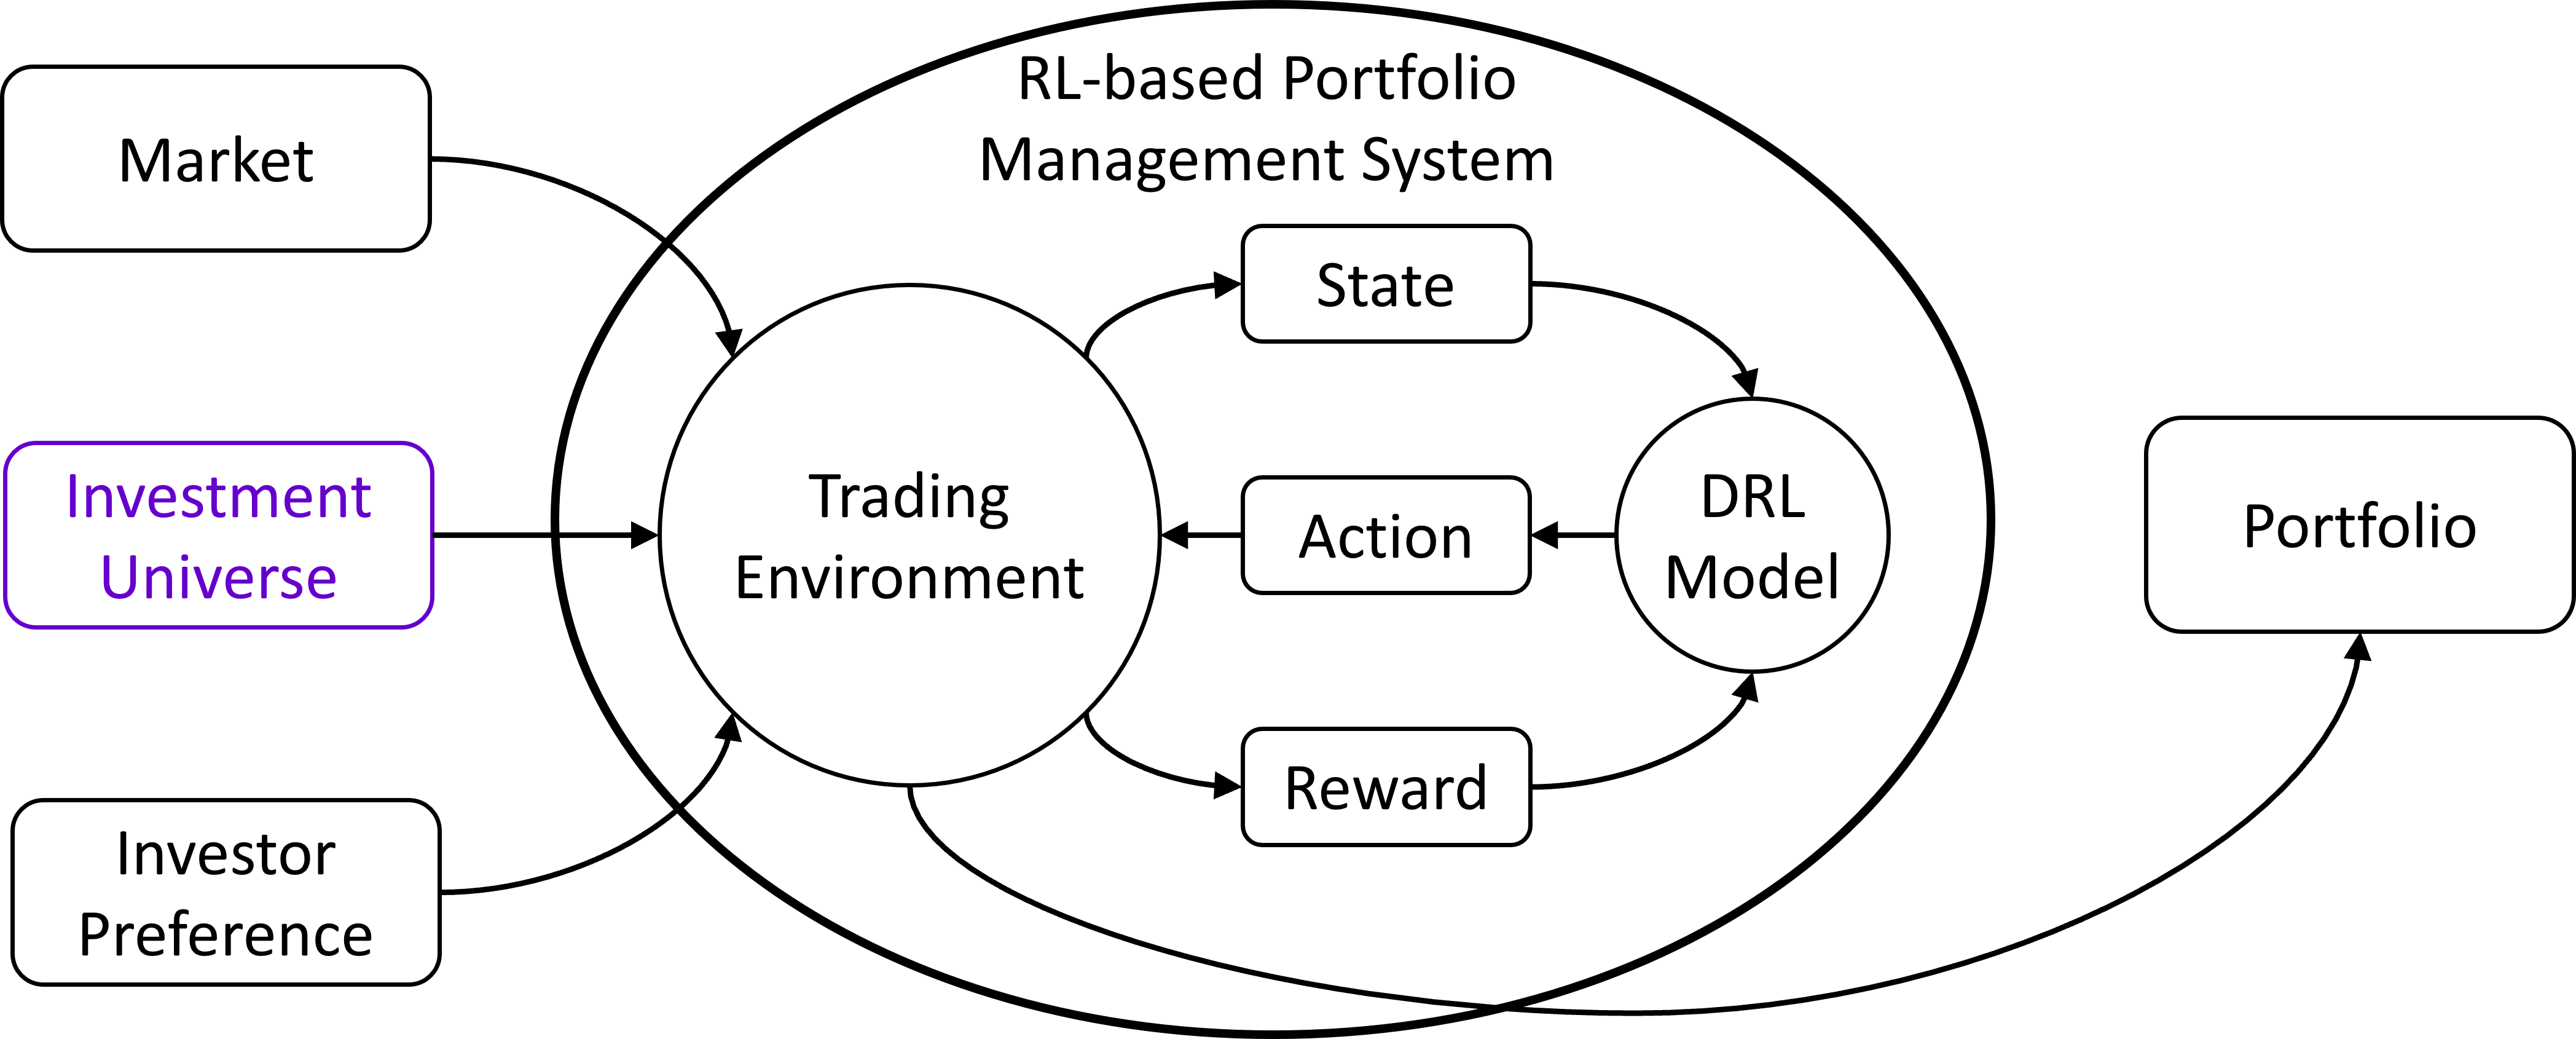
\includegraphics[width=10cm]{images/investment_universe.png}
\end{frame}

\begin{frame}{Investment Universe}
\begin{block}{Goal}
\begin{itemize}
    \item Choose 10 investments
    \item Low covariances between each other
\end{itemize}
\end{block}
\begin{block}{Selection Process}
    \begin{enumerate}
    \item Starts from the top 100 ETFs by Asset Under Management (AUM)
    \item Remove ones with trading records of less than 14 years.
    \item \label{itm:remove_items} Obtain the top two most correlated ETFs and remove the one with lower AUM
    \item Repeat \mynum{\ref{itm:remove_items}} iteratively until 10 ETFs are left
    \end{enumerate}
\end{block}
\end{frame}

\begin{frame}{Selection of ETFs}
    \begin{tabular}{|| c | c ||}
    \hline
    Symbol & Name  \\ \hline \hline
    SPY&SPDR S\&P 500 ETF \\ \hline
    AGG&iShares Core U.S. Aggregate Bond ETF \\ \hline
    BND&Vanguard Total Bond Market ETF \\ \hline
    GLD&SPDR Gold Trust \\ \hline
    LQD&iShares iBoxx \$ Investment Grade Corporate Bond ETF \\ \hline
    BSV&Vanguard Short-Term Bond ETF \\ \hline
    MBB&iShares MBS Bond ETF \\ \hline
    IGSB&iShares Short-Term Corporate Bond ETF \\ \hline
    SHY&iShares 1-3 Year Treasury Bond ETF \\ \hline
    SHV&iShares Short Treasury Bond ETF \\ \hline
    \end{tabular}
\end{frame}

\begin{frame}{Risk and Return of selected ETFs}
\centering
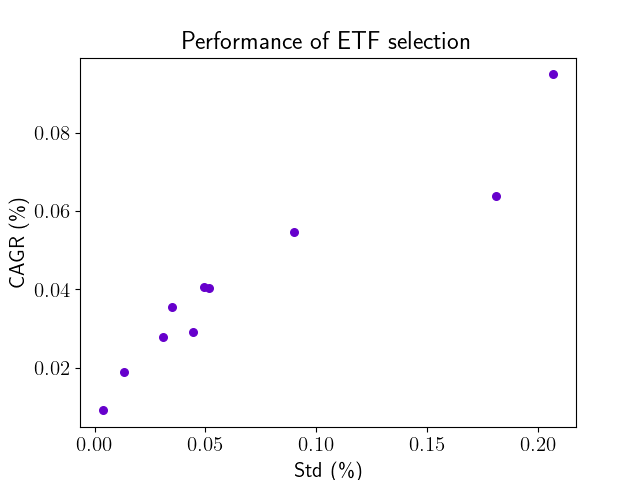
\includegraphics[width=10cm]{images/etfs.png}
\end{frame}

\subsection{Investor Preference}
\begin{frame}{Investor Preference}
    \begin{block}{Objective}
        Define indicator to represent investor preference.
    \end{block}
\centering
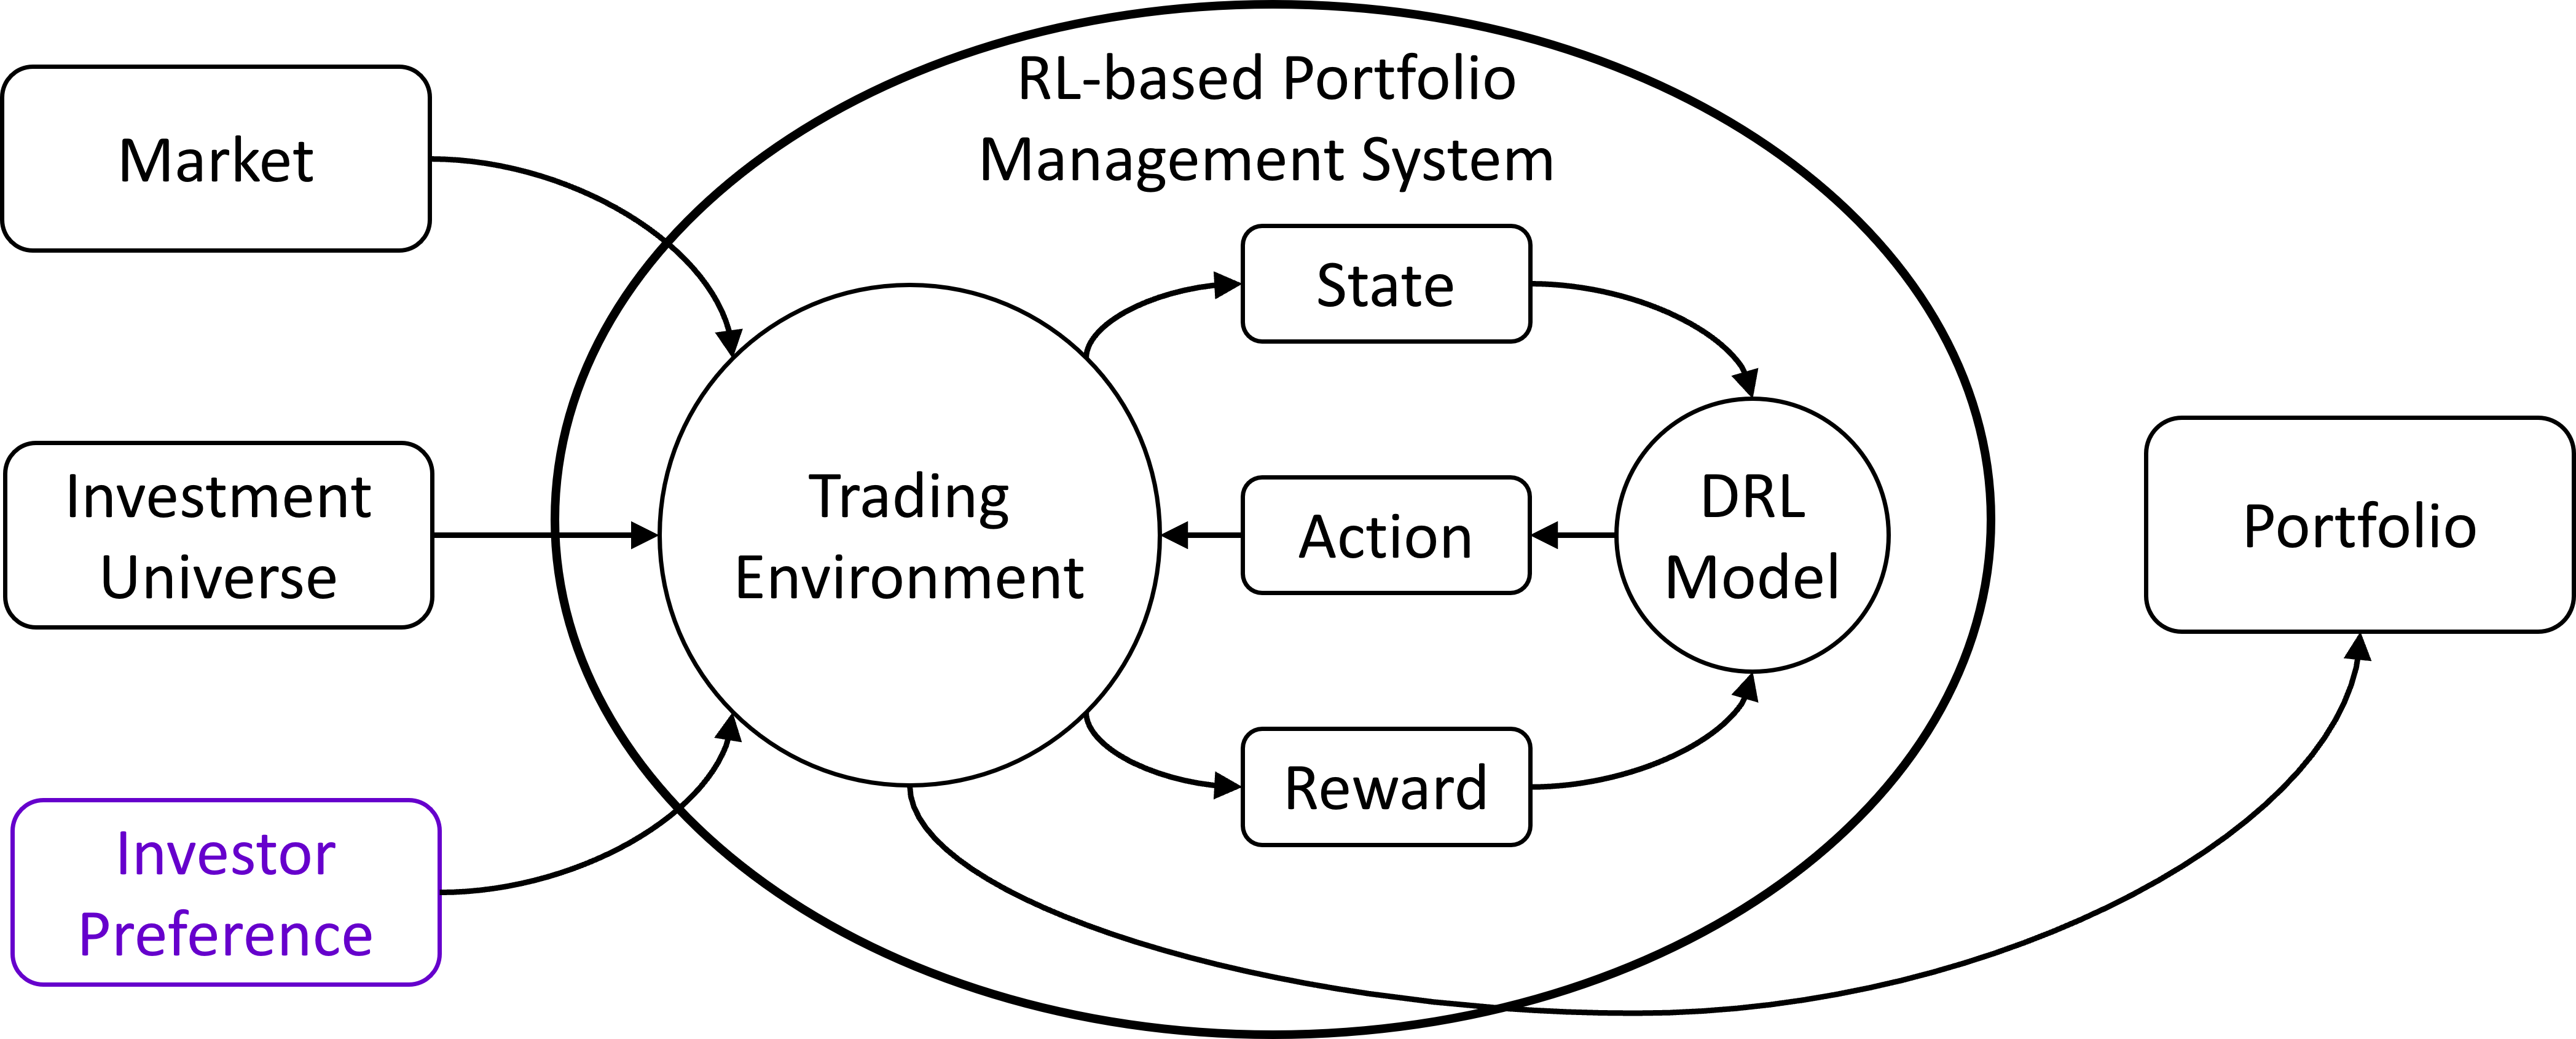
\includegraphics[width=10cm]{images/investor_preference.png}
\end{frame}

\begin{frame}{Investor Preference}
\begin{block}{Risk Preference Acquisition}
\begin{itemize}
    \item Acquire risk preference from investors by survey or other techniques and interprets into indicators.
    \item \alert{This part is not in the scope of our thesis}
\end{itemize}

\end{block}
\begin{block}{Standard Deviation}
\begin{itemize}
    \item Sharpe Ratio uses the standard deviation to represent a risk
    \item \alert{Blooming return also yield a high standard deviation}
\end{itemize}
\end{block}
\begin{block}{Maximum Drawdown (MDD)}
\begin{itemize}
    \item The decline from the highest peak.
    \item \alert{Challenge to optimize}
    \item Used for performance evaluation not for optimizing
\end{itemize}
\end{block}
\end{frame}



\subsection{Portfolio}


\begin{frame}{Portfolio}
    \begin{block}{Objective}
        Define a data structure to represent portfolio.
    \end{block}
\centering
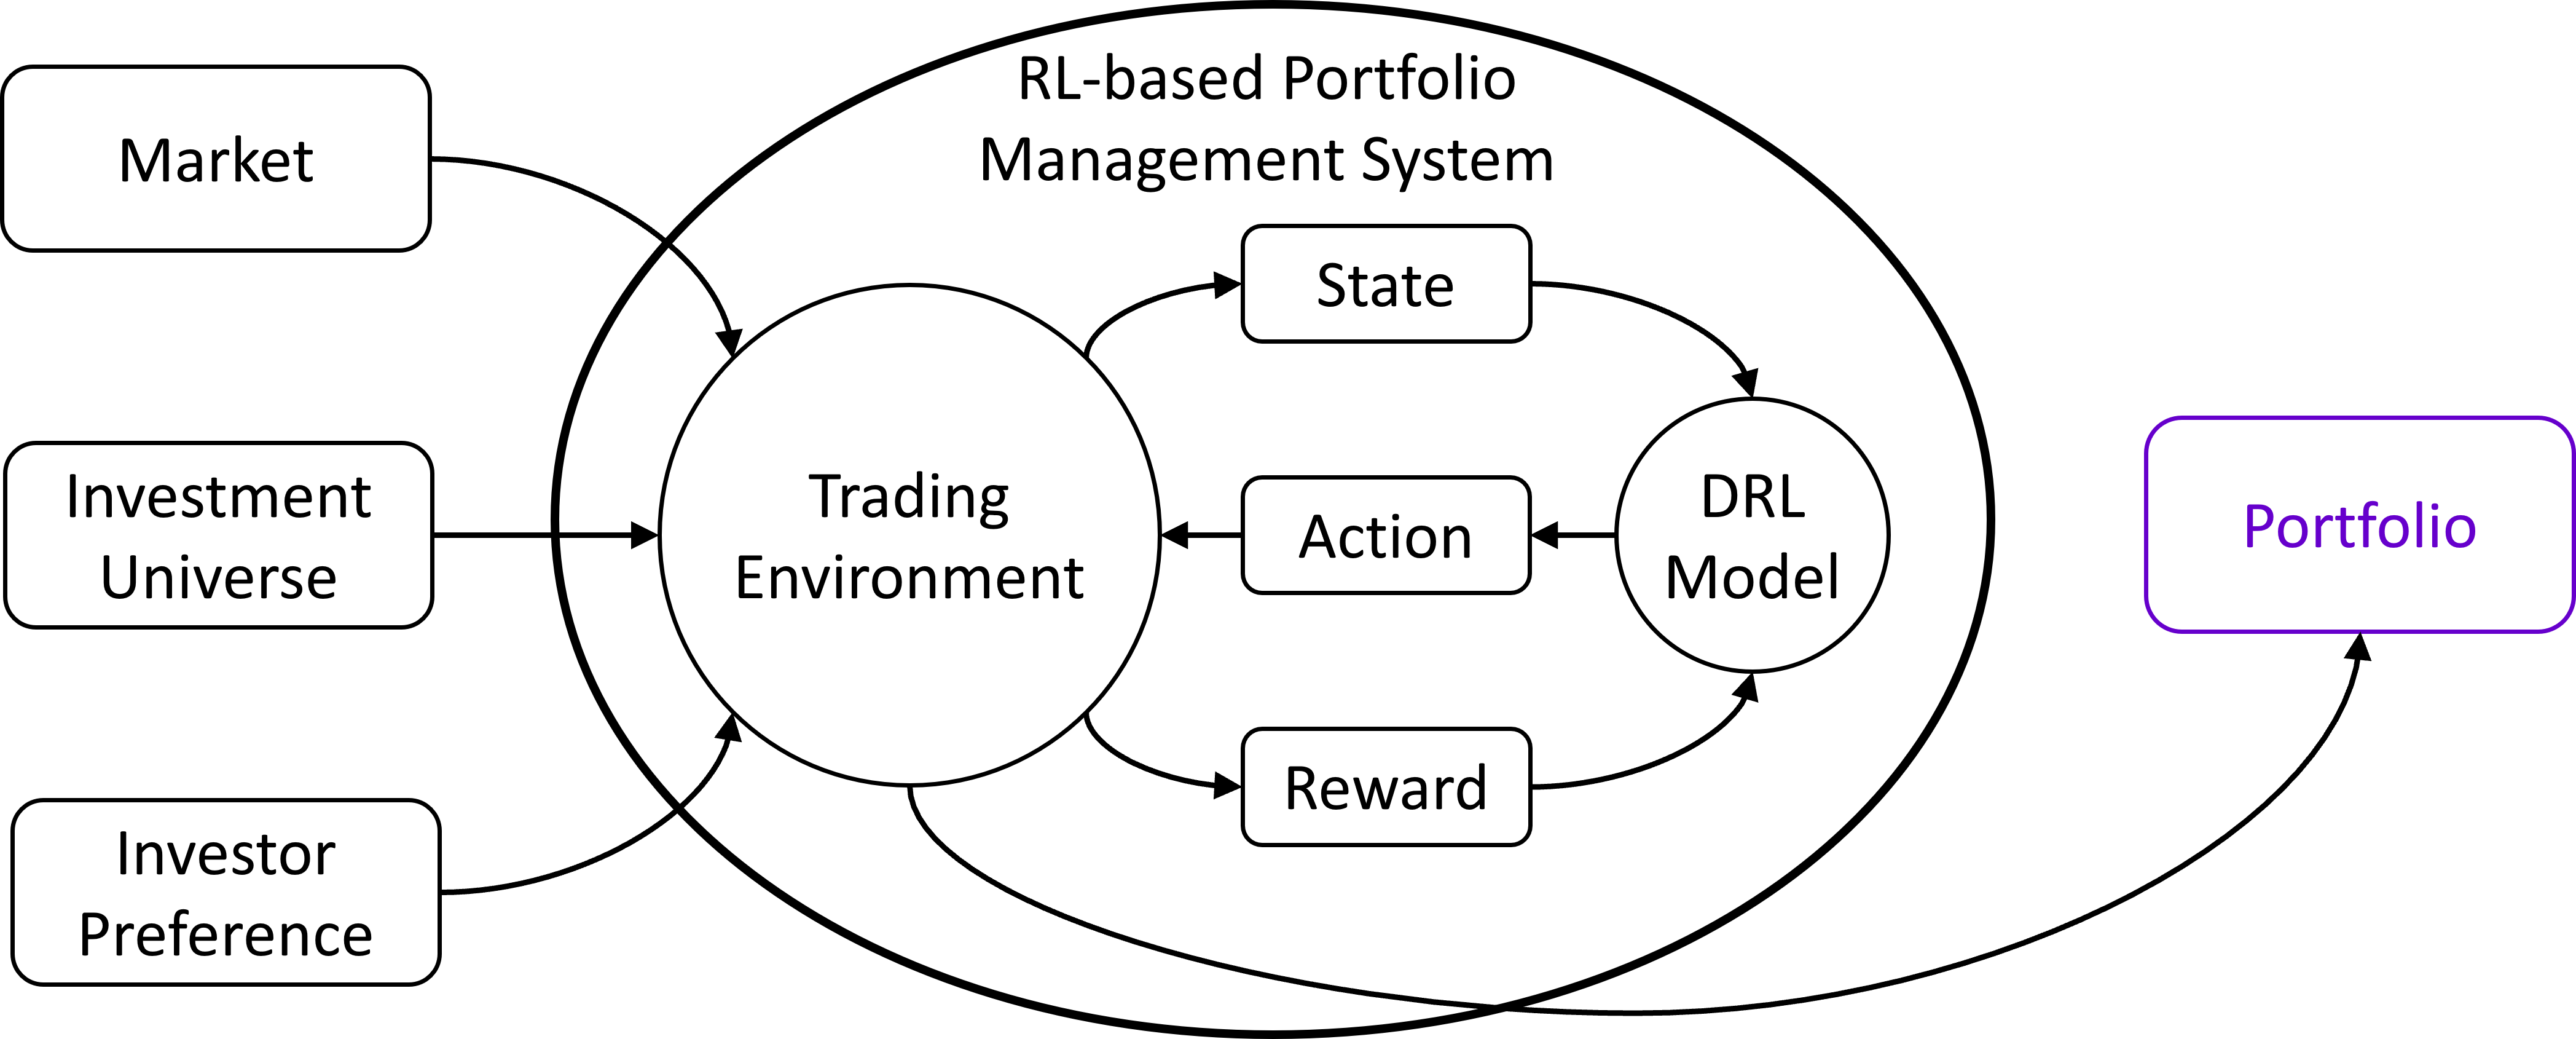
\includegraphics[width=10cm]{images/portfolio.png}

\end{frame}



\begin{frame}{Portfolio}
\begin{block}{Portfolio}
The portfolio F is an m dimension vector space of weights f.
\[
    F = \{ {f \in \mathbb{R} } \} ^m,
    \sum_{i=1}^m {f_i} =1
\]
\end{block}
\begin{block}{Weight}
Weight is a real number between 0 and 1. \alert{(No short position)}
\[
    f \in \mathbb{R} | 0 \leq f \leq 1 
\]
\end{block}
\end{frame}
